\documentclass[aspectratio=169]{beamer}

\usetheme{Madrid}
\usecolortheme{default}
\usefonttheme{professionalfonts}

\usepackage[utf8]{inputenc}
\usepackage[T1]{fontenc}
\usepackage[indonesian]{babel}
\usepackage{amsmath}
\usepackage{booktabs}
\usepackage{graphicx}
\usepackage{array}
\usepackage{xcolor}
\usepackage{listings}
\usepackage{bytefield}

% ── listing style for inline code blocks ──────────────────────
\lstset{
  basicstyle=\ttfamily\scriptsize,
  breaklines=true,
  frame=single,
  backgroundcolor=\color{gray!10},
  keywordstyle=\color{blue},
  commentstyle=\color{green!50!black},
  stringstyle=\color{red!70!black},
}

% ── colour shortcuts ──────────────────────────────────────────
\newcommand{\good}[1]{\textcolor{green!60!black}{\textbf{#1}}}
\newcommand{\bad}[1]{\textcolor{red!70!black}{\textbf{#1}}}
\newcommand{\reg}[1]{\texttt{\small #1}}

\title{Perancangan IP I2S TX AXI4-Lite\\pada SoC MicroBlaze V}
\subtitle{Implementasi pada FPGA Basys3 dengan DAC PCM5102A\\
          \small Termasuk Identifikasi dan Perbaikan Bug Firmware}
\author{Nama Mahasiswa \\ NIM}
\institute{Departemen Teknik Elektro dan Teknologi Informasi\\Universitas Gadjah Mada}
\date{Mei 2026}

\begin{document}

% ── TITLE ─────────────────────────────────────────────────────
\begin{frame}
  \titlepage
\end{frame}

% ── OUTLINE ───────────────────────────────────────────────────
\begin{frame}{Outline}
  \tableofcontents
\end{frame}

%==============================================================
\section{Pendahuluan}
%==============================================================

\begin{frame}{Latar Belakang}
  \begin{itemize}
    \item Sistem embedded audio membutuhkan antarmuka serial yang \textbf{stabil, presisi,
          dan dapat dikonfigurasi dari perangkat lunak}.
    \item \textbf{I2S} (Philips, 1986) adalah standar de-facto untuk transmisi audio
          digital antarchip: BCLK, WS/LRCK, DATA.
    \item \textbf{AXI4-Lite} memungkinkan prosesor mengakses register peripheral
          melalui model \textit{memory-mapped I/O} yang sederhana.
    \item \textbf{MicroBlaze V} (RISC-V soft-core) pada ekosistem AMD/Xilinx
          menyediakan fondasi SoC yang terintegrasi dengan Vivado dan Vitis.
    \item Penelitian ini merancang IP I2S TX kustom, mengintegrasikannya ke SoC,
          \textbf{dan mendokumentasikan bug firmware} yang ditemukan selama validasi.
  \end{itemize}
\end{frame}

\begin{frame}{Rumusan Masalah dan Tujuan}
  \begin{columns}[T]
    \column{0.5\textwidth}
      \textbf{Rumusan Masalah}
      \begin{enumerate}\small
        \item Bagaimana merancang IP I2S TX dengan AXI4-Lite yang
              dapat diakses melalui register \textit{memory-mapped}?
        \item Bagaimana mendukung dua mode $F_s$ (48/96 kHz) dari
              satu sumber \texttt{audio\_clk}?
        \item Bagaimana memverifikasi fungsionalitas dan timing
              melalui ILA dan uji audio PCM5102A?
      \end{enumerate}
    \column{0.5\textwidth}
      \textbf{Batasan Penelitian}
      \begin{itemize}\small
        \item TX-only, format Philips I2S, stereo.
        \item Bare-metal (tanpa RTOS/Linux).
        \item Tanpa DMA dan tanpa FIFO internal.
        \item Platform: Basys3 (Artix-7) + PCM5102A.
        \item \textit{Programmed I/O} berbasis register murni.
      \end{itemize}
  \end{columns}
\end{frame}

%==============================================================
\section{Dasar Teori}
%==============================================================

\begin{frame}{Protokol I2S -- Philips Standard}
  \begin{columns}[T]
    \column{0.55\textwidth}
      \begin{itemize}
        \item \textbf{BCLK}: clock serial, \textit{sampling} data pada tepi naik.
        \item \textbf{WS}: LOW = kanal kiri; HIGH = kanal kanan.
        \item \textbf{DATA}: serial MSB-first; satu \textbf{delay bit} (selalu 0)
              setelah setiap peralihan WS.
        \item Satu frame stereo = \textbf{64 BCLK}
              (32 bit kiri + 32 bit kanan).
        \item DATA berubah pada tepi \textit{turun} BCLK; DAC membaca
              pada tepi \textit{naik}.
      \end{itemize}
    \column{0.45\textwidth}
      \IfFileExists{contents/figures/diagram-sinyal-i2s-philips.pdf}{%
        \includegraphics[width=\linewidth]{contents/figures/diagram-sinyal-i2s-philips.pdf}%
      }{}
  \end{columns}
\end{frame}

\begin{frame}{Relasi Clock I2S}
  \[
    F_s = \frac{f_{\mathrm{audio\_clk}}}{\mathrm{divider} \times 2 \times 64}
  \]
  \vspace{0.4em}
  \begin{center}
  \small
  \begin{tabular}{lcccc}
    \toprule
    Mode & $f_{\mathrm{audio\_clk}}$ req. & $f_{\mathrm{audio\_clk}}$ aktual
         & Divider & $F_s$ aktual \\
    \midrule
    \texttt{FS\_MODE=0} & 24,576 MHz & 24,597 MHz & 8 & \good{48,03 kHz} \\
    \texttt{FS\_MODE=1} & 24,576 MHz & 24,597 MHz & 4 & \good{96,08 kHz} \\
    \bottomrule
  \end{tabular}
  \end{center}
  \vspace{0.3em}
  \begin{itemize}\small
    \item \texttt{FS\_FAMILY=0}: gunakan \texttt{audio\_48\_clk} (24,597 MHz).
    \item \texttt{FS\_FAMILY=1}: gunakan \texttt{audio\_44\_clk} (22,426 MHz)
          untuk keluarga 44,1/88,2 kHz.
  \end{itemize}
\end{frame}

%==============================================================
\section{Perancangan Sistem}
%==============================================================

\begin{frame}{Arsitektur Sistem -- Block Design}
  \begin{columns}[T]
    \column{0.50\textwidth}
      \begin{itemize}
        \item \textbf{MicroBlaze V} sebagai AXI master.
        \item \textbf{AXI SmartConnect} menghubungkan prosesor ke peripheral.
        \item \textbf{Clocking Wizard} menghasilkan 3 clock:\\
              100 MHz (AXI), 24,6 MHz (48k), 22,4 MHz (44,1k).
        \item \textbf{IP I2S} menerima data lewat register AXI4-Lite.
        \item Output PMOD JA → \textbf{PCM5102A}.
      \end{itemize}
    \column{0.50\textwidth}
      \IfFileExists{contents/figures/block-design-vivado-i2s-screenshot.png}{%
        \includegraphics[width=\linewidth]{contents/figures/block-design-vivado-i2s-screenshot.png}%
      }{}
  \end{columns}
\end{frame}

\begin{frame}{Arsitektur Internal IP I2S TX}
  \begin{columns}[T]
    \column{0.50\textwidth}
      \textbf{5 bagian utama RTL:}
      \begin{enumerate}\small
        \item \textbf{AXI4-Lite slave} -- register write/read state machine.
        \item \textbf{CDC write-counter} -- sinkronisasi 2-FF dari domain AXI ke domain audio.
        \item \textbf{BUFGMUX} -- pilih \texttt{audio\_48\_clk} atau \texttt{audio\_44\_clk}.
        \item \textbf{Clock divider} -- \texttt{bclk\_en\_w} setiap 4 atau 8 siklus MCLK.
        \item \textbf{Serializer} -- Philips I2S, delay-bit, MSB-first, lebar variabel.
      \end{enumerate}
    \column{0.50\textwidth}
      \IfFileExists{contents/figures/block-diagram-ip-i2s-tx-intern.pdf}{%
        \includegraphics[width=\linewidth]{contents/figures/block-diagram-ip-i2s-tx-intern.pdf}%
      }{}
  \end{columns}
\end{frame}

\begin{frame}{Register Map IP I2S}
  \begin{center}
  \small
  \begin{tabular}{>{\ttfamily}l l p{6.2cm}}
    \toprule
    Offset & Nama & Fungsi \\
    \midrule
    0x00 & DATA\_LEFT  & Sampel kanal kiri; MSB di bit [\texttt{SAMPLE\_WIDTH}-1] \\
    0x04 & DATA\_RIGHT & Sampel kanal kanan; packing sama dengan kiri \\
    0x08 & CONTROL     & Enable, Mute, FS\_FAMILY, FS\_MODE, SAMPLE\_WIDTH \\
    0x0C & RESERVED    & Scratch (dipakai readback test AXI) \\
    \bottomrule
  \end{tabular}
  \end{center}

  \vspace{0.5em}
  \textbf{Bitfield CONTROL:}
  \begin{center}
  \scriptsize
  \begin{tabular}{cll}
    \toprule
    Bit & Field & Keterangan \\
    \midrule
    0 & ENABLE & 1 = output aktif \\
    1 & MUTE & 1 = paksa DATA = 0 (clock tetap) \\
    2 & FS\_FAMILY & 0 = 48/96 kHz; 1 = 44,1/88,2 kHz \\
    3 & FS\_MODE & 0 = Fs rendah; 1 = Fs tinggi (×2) \\
    12:8 & SAMPLE\_WIDTH & Lebar bit per kanal (0 → default 32) \\
    \bottomrule
  \end{tabular}
  \end{center}
\end{frame}

\begin{frame}{Constraint dan Wiring PCM5102A}
  \begin{columns}[T]
    \column{0.50\textwidth}
      \textbf{Pemetaan pin (cnstr.xdc):}
      \begin{center}\scriptsize
      \begin{tabular}{ll}
        \toprule
        Sinyal & PMOD JA Pin \\
        \midrule
        \texttt{i2s\_mclk} & J1 \\
        \texttt{i2s\_bclk} & L2 \\
        \texttt{i2s\_ws}   & J2 \\
        \texttt{i2s\_data} & G2 \\
        \bottomrule
      \end{tabular}
      \end{center}
      \vspace{0.4em}
      Semua pin \texttt{LVCMOS33}, cocok dengan tegangan kerja PCM5102A.
    \column{0.50\textwidth}
      \IfFileExists{contents/figures/pmod-pcm-wiring-diagram.png}{%
        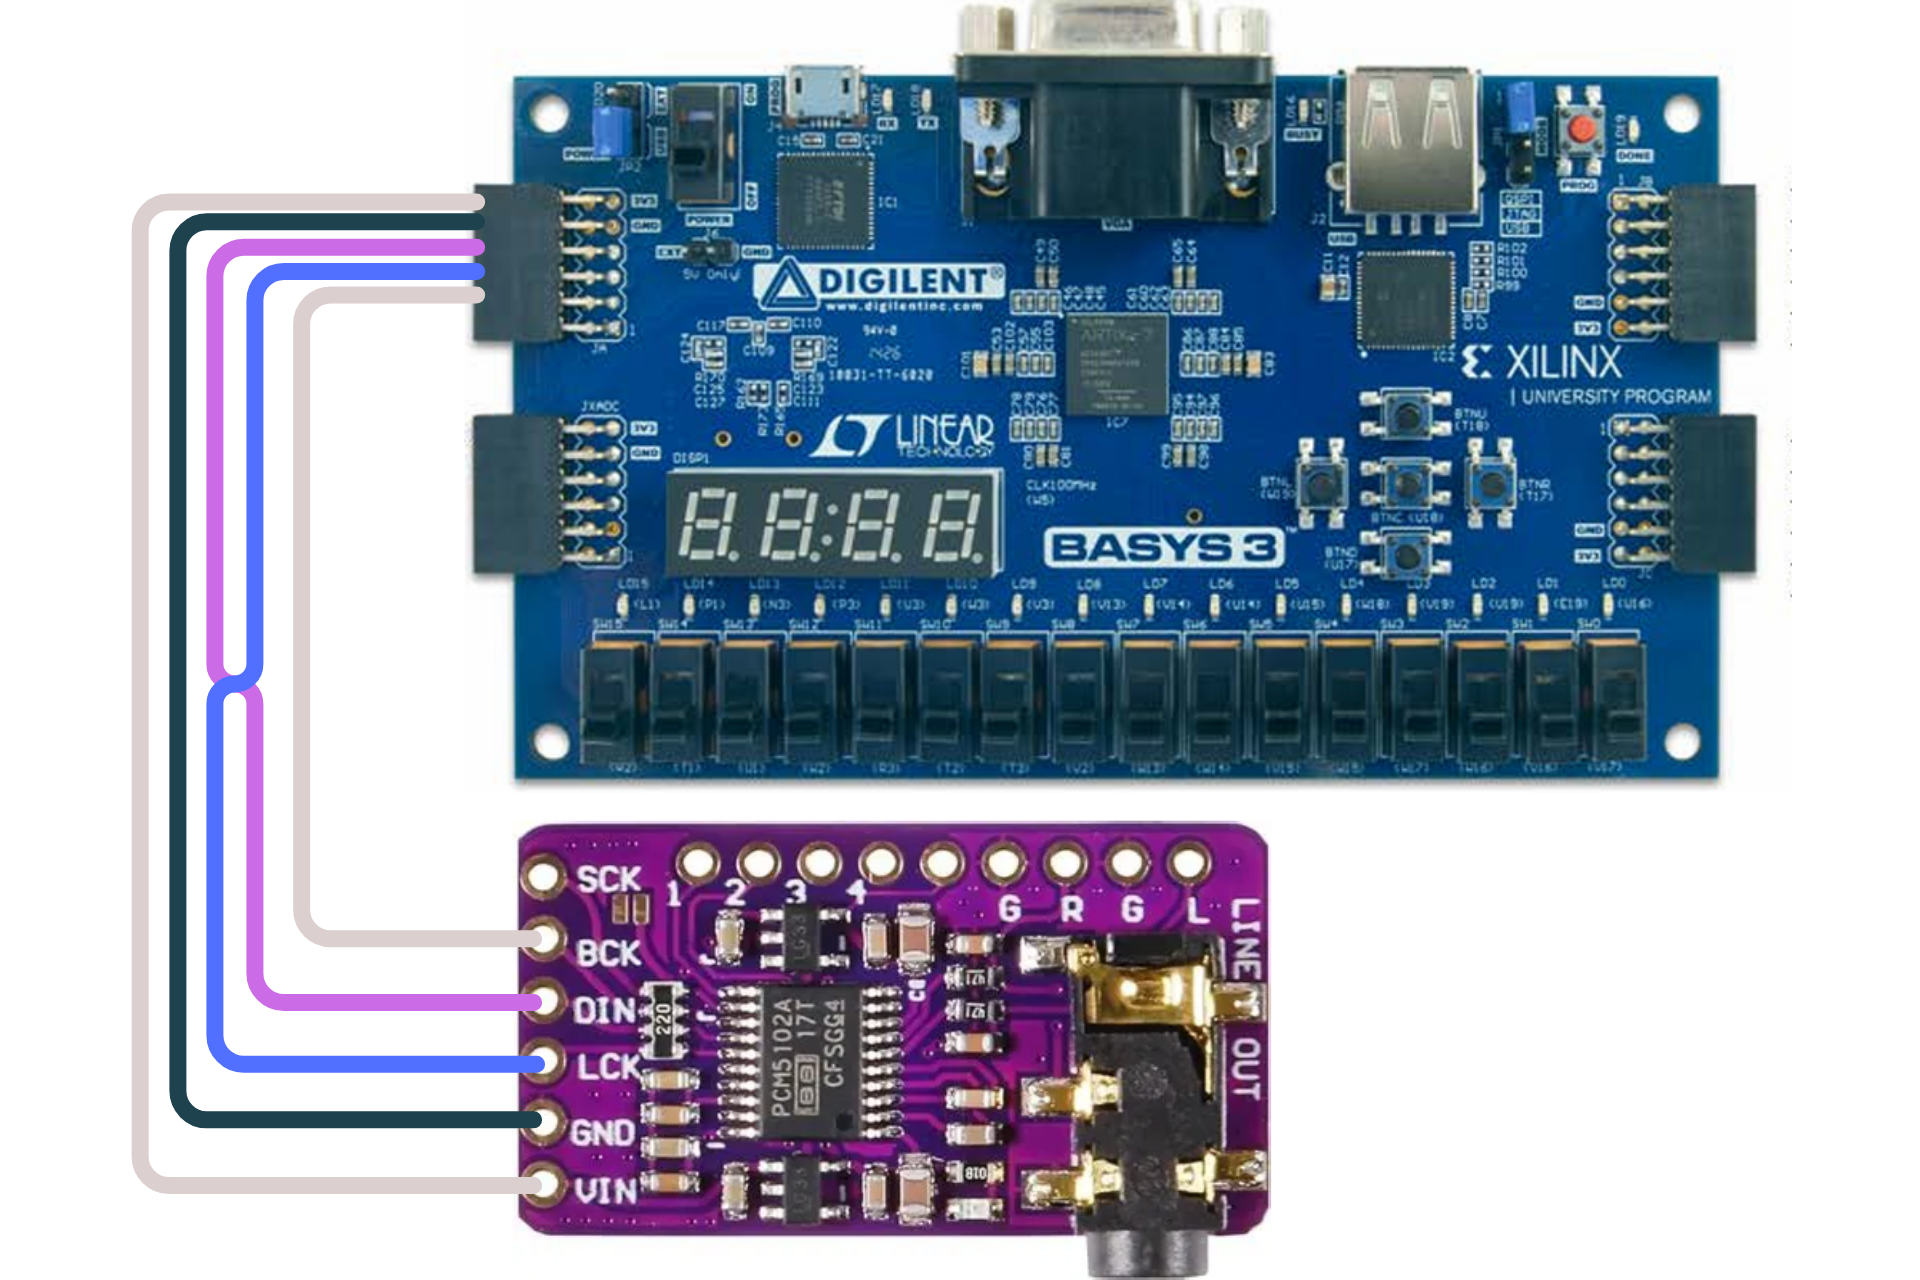
\includegraphics[width=\linewidth]{contents/figures/pmod-pcm-wiring-diagram.png}%
      }{}
  \end{columns}
\end{frame}

%==============================================================
\section{Implementasi Firmware}
%==============================================================

\begin{frame}{Aplikasi Vitis -- Alur Utama}
  \begin{enumerate}
    \item Tulis register \texttt{CONTROL} (ENABLE=1, SAMPLE\_WIDTH=24, mode clock).
    \item Loop utama: hitung sampel sinus $\rightarrow$ tulis \texttt{DATA\_LEFT} \&
          \texttt{DATA\_RIGHT} $\rightarrow$ tunggu deadline.
    \item Poll UART untuk perintah keyboard (frekuensi, kanal, mute, dll.).
  \end{enumerate}

  \vspace{0.5em}
  \textbf{Fitur yang dapat dikontrol dari terminal:}
  \begin{center}\small
  \begin{tabular}{cl}
    \toprule
    Tombol & Fungsi \\
    \midrule
    \texttt{1/2/5} & Pilih frekuensi 1 kHz / 2 kHz / 5 kHz \\
    \texttt{L/R/B} & Pilih kanal Left / Right / Both \\
    \texttt{M} & Toggle MUTE \\
    \texttt{E} & Toggle ENABLE \\
    \texttt{W} & Siklus SAMPLE\_WIDTH: 16 → 24 → 32 → 16 \\
    \texttt{F/O} & Toggle FS\_FAMILY / FS\_MODE \\
    \bottomrule
  \end{tabular}
  \end{center}
\end{frame}

%==============================================================
\section{Identifikasi dan Perbaikan Bug}
%==============================================================

\begin{frame}{Gejala yang Ditemukan}
  \begin{center}
  \small
  \begin{tabular}{clll}
    \toprule
    \# & Gejala & Kondisi & Bukan dari RTL? \\
    \midrule
    1 & Kedua kanal mute & Mode Both aktif & \good{Ya} \\
    2 & Kanal kanan mute & Mode Right-only & \good{Ya} \\
    3 & Amplitudo L $\neq$ R & Both aktif & \good{Ya} \\
    4 & Semua frekuensi lebih rendah & 1k/2k/5kHz & \good{Ya} \\
    5 & 32-bit bersuara salah & SAMPLE\_WIDTH=32 & \good{Ya} \\
    \bottomrule
  \end{tabular}
  \end{center}

  \vspace{0.5em}
  \begin{alertblock}{Temuan kunci}
    Seluruh 5 gejala bersumber dari \textbf{kode firmware} (\texttt{helloworld.c}),
    bukan dari RTL. RTL terbukti benar sejak awal.
  \end{alertblock}
\end{frame}

\begin{frame}[fragile]{Bug 1 \& 2: Masker Merusak Bit Tanda Sampel}
  \textbf{Penyebab:} masker menghapus bit tanda sampel negatif setelah geseran.

  \begin{columns}[T]
    \column{0.50\textwidth}
      \textbf{\bad{Kode lama (salah):}}
\begin{lstlisting}[language=C]
// untuk 24-bit: mask = 0x00FFFFFF
uint32_t mask = (1U << g_width) - 1U;
uint32_t samp = (uint32_t)s32 & mask;
// bit tanda [31:24] ikut terpotong!
\end{lstlisting}

    \column{0.50\textwidth}
      \textbf{\good{Kode baru (benar):}}
\begin{lstlisting}[language=C]
// RTL hanya baca [width-1:0]
// tidak perlu masker sama sekali
int32_t s32;
if      (g_width >= 32) s32 = (int32_t)s << 16;
else if (g_width >  16) s32 = (int32_t)s << (g_width-16);
else if (g_width <  16) s32 = (int32_t)s >> (16-g_width);
else                    s32 = (int32_t)s;
uint32_t samp = (uint32_t)s32; // tanpa mask
\end{lstlisting}
  \end{columns}

  \vspace{0.4em}
  \textbf{Aturan justifikasi:} geser int16 sehingga MSB-nya tepat di bit \texttt{[SAMPLE\_WIDTH-1]}.
  \begin{center}\small
  \begin{tabular}{ccc}
    \toprule
    SAMPLE\_WIDTH & Geseran & MSB di bit \\
    \midrule
    16 & 0 & 15 \\
    24 & $\ll$ 8 & 23 \\
    32 & $\ll$ 16 & 31 \\
    \bottomrule
  \end{tabular}
  \end{center}
\end{frame}

\begin{frame}[fragile]{Bug 3: Frekuensi Lebih Rendah dari Target}
  \textbf{Penyebab:} \texttt{usleep(periode - 2)} tidak akumulatif dan tidak presisi.

  \begin{columns}[T]
    \column{0.48\textwidth}
      \textbf{\bad{Kode lama:}}
\begin{lstlisting}[language=C]
uint32_t period_us =
  (1000000U + sr/2U) / sr;
usleep(period_us - 2);
// -2 adalah tebakan
// error terakumulasi tiap iterasi
// di 96kHz: 10us - 2 = 8us → 20% off
\end{lstlisting}

    \column{0.52\textwidth}
      \textbf{\good{Kode baru (deadline absolut):}}
\begin{lstlisting}[language=C]
// rdcycle64(): baca CSR mcycle RISC-V
// resolusi 10 ns pada 100 MHz CPU
uint64_t deadline = rdcycle64();
while (1) {
  uint64_t period =
    100000000ULL / current_sample_rate();
  stream_sample();
  poll_uart();
  deadline += period; // maju tepat 1 periode
  while (rdcycle64() < deadline) {}
}
\end{lstlisting}
  \end{columns}

  \vspace{0.3em}
  \begin{block}{Keunggulan deadline-based}
    \small Overhead loop (AXI write, UART poll) dikompensasi otomatis.
    Presisi setara osilator 100 MHz board -- tidak ada drift kumulatif.
  \end{block}
\end{frame}

\begin{frame}{Perbandingan Metode Timing Loop}
  \begin{center}
  \begin{tabular}{lcc}
    \toprule
    Properti & \bad{usleep() lama} & \good{rdcycle64() baru} \\
    \midrule
    Resolusi waktu & $\approx$1 µs & 10 ns \\
    Kompensasi overhead loop & Tebakan (-2 µs) & Otomatis \\
    Akumulasi error & \bad{Ya} & \good{Tidak} \\
    Bekerja di 96 kHz (10,4 µs/sampel) & \bad{Tidak ($\approx$20\% off)} & \good{Ya} \\
    Header tambahan dibutuhkan & Tidak & Tidak \\
    \bottomrule
  \end{tabular}
  \end{center}

  \vspace{0.5em}
  \begin{itemize}\small
    \item \texttt{rdcycle}/\texttt{rdcycleh} adalah instruksi CSR standar RISC-V,
          tersedia pada MicroBlaze V tanpa header khusus.
    \item Loop ganda (\textit{read-hi, read-lo, read-hi}) mencegah race condition
          saat carry dari bit 31 ke bit 32.
  \end{itemize}
\end{frame}

%==============================================================
\section{Hasil Pengujian}
%==============================================================

\begin{frame}{Hasil ILA -- Verifikasi Timing I2S}
  \begin{columns}[T]
    \column{0.50\textwidth}
      \textbf{Yang dikonfirmasi:}
      \begin{itemize}\small
        \item 64 BCLK per frame stereo ✓
        \item WS beralih 1 BCLK \textit{sebelum} MSB ✓
        \item Bit pertama setelah WS selalu 0 (delay bit) ✓
        \item BCLK = 3,0746 MHz ✓
        \item WS = 48,03 kHz ✓
        \item Kedua kanal L dan R aktif ✓
      \end{itemize}
    \column{0.50\textwidth}
      \IfFileExists{contents/figures/ila-bclk-ws-data.png}{%
        \includegraphics[width=\linewidth]{contents/figures/ila-bclk-ws-data.png}%
      }{}
  \end{columns}
\end{frame}

\begin{frame}{Hasil Verifikasi Firmware Setelah Perbaikan}
  \begin{center}
  \small
  \begin{tabular}{llc}
    \toprule
    Skenario Uji & Hasil yang Diharapkan & Status \\
    \midrule
    Both + 1 kHz  & L dan R identik, 1 kHz  & \good{\checkmark} \\
    Left only     & L aktif, R = 0           & \good{\checkmark} \\
    Right only    & R aktif, L = 0           & \good{\checkmark} \\
    Both + 2 kHz  & L dan R identik, 2 kHz  & \good{\checkmark} \\
    Both + 5 kHz  & L dan R identik, 5 kHz  & \good{\checkmark} \\
    MUTE aktif    & Diam, BCLK/WS tetap     & \good{\checkmark} \\
    WIDTH = 16 bit & Amplitudo benar         & \good{\checkmark} \\
    WIDTH = 32 bit & Amplitudo penuh, benar  & \good{\checkmark} \\
    \bottomrule
  \end{tabular}
  \end{center}
\end{frame}

\begin{frame}{Verifikasi Audio PCM5102A}
  \begin{columns}[T]
    \column{0.50\textwidth}
      \begin{itemize}\small
        \item Sinyal sinus 1 kHz, 2 kHz, dan 5 kHz terdengar jelas
              melalui speaker/headphone.
        \item Mode Both: L dan R \textbf{amplitudo identik}.
        \item Mode Left/Right: kanal inaktif benar-benar senyap.
        \item Mode Mute: tidak ada suara, BCLK/WS tetap berjalan
              (DAC tetap terkunci pada clock).
      \end{itemize}
    \column{0.50\textwidth}
      \IfFileExists{contents/figures/scope-sine-both-ch-fixed.png}{%
        \includegraphics[width=\linewidth]{contents/figures/scope-sine-both-ch-fixed.png}%
      }{}
  \end{columns}
\end{frame}

\begin{frame}{Ringkasan Analisis Frekuensi}
  \begin{center}
  \small
  \begin{tabular}{lccc}
    \toprule
    Besaran & Target nominal & Hasil (clock aktual) & Selisih \\
    \midrule
    $f_{\mathrm{audio\_clk}}$ 48k & 24,576 MHz & 24,597 MHz & +0,09\% \\
    BCLK (\texttt{FS\_MODE=0}) & 3,072 MHz & 3,0746 MHz & +0,08\% \\
    $F_s$ (\texttt{FS\_MODE=0}) & 48,000 kHz & 48,03 kHz & +0,06\% \\
    BCLK (\texttt{FS\_MODE=1}) & 6,144 MHz & 6,1493 MHz & +0,08\% \\
    $F_s$ (\texttt{FS\_MODE=1}) & 96,000 kHz & 96,08 kHz & +0,08\% \\
    \bottomrule
  \end{tabular}
  \end{center}

  \vspace{0.4em}
  \begin{itemize}\small
    \item Selisih $<$0,1\% -- berasal dari keterbatasan rasio MMCM Artix-7,
          bukan dari bug.
    \item Kedua mode $F_s$ tervalidasi setelah bug firmware timing diperbaiki.
  \end{itemize}
\end{frame}

%==============================================================
\section{Penutup}
%==============================================================

\begin{frame}{Kesimpulan}
  \begin{enumerate}
    \item \textbf{IP I2S TX AXI4-Lite} berhasil dirancang dan diintegrasikan
          pada SoC MicroBlaze V di Basys3 dengan register map aktif
          (\texttt{0x00}, \texttt{0x04}, \texttt{0x08}).

    \item \textbf{Dua mode $F_s$} (48,03 kHz dan 96,08 kHz) berhasil dihasilkan
          dari satu \texttt{audio\_48\_clk} (24,597 MHz) melalui divider 8 dan 4.

    \item \textbf{Timing I2S} terverifikasi via ILA: 64 BCLK/frame, delay-bit
          wajib, WS sesuai spesifikasi Philips.

    \item \textbf{Tiga bug firmware} ditemukan dan diperbaiki \textit{sepenuhnya
          di sisi software} -- RTL tidak dimodifikasi:
          \begin{itemize}\small
            \item Masker merusak bit tanda sampel negatif.
            \item Justifikasi sampel 32-bit tidak tepat (MSB salah posisi).
            \item Loop timing \texttt{usleep} tidak akumulatif; diganti
                  \texttt{rdcycle64()} dengan presisi 10 ns.
          \end{itemize}

    \item \textbf{Validasi audio PCM5102A} berhasil: L = R amplitudo identik,
          seleksi kanal berfungsi, frekuensi 1/2/5 kHz terukur benar.
  \end{enumerate}
\end{frame}

\begin{frame}{Saran Pengembangan}
  \begin{enumerate}
    \item Menambahkan \textbf{FIFO TX} dan \textbf{watermark interrupt} untuk
          mengurangi beban CPU dan mencegah \textit{underrun} pada beban tinggi.
    \item Mengintegrasikan \textbf{DMA} untuk \textit{streaming} audio kontinu
          tanpa keterlibatan CPU per sampel.
    \item Menambahkan register \textbf{STATUS} (level buffer, flag underrun)
          untuk mendukung pengembangan driver berbasis OS.
    \item Mengembangkan mode \textbf{RX} atau ekstensi \textbf{TDM/multi-channel}
          untuk sistem akuisisi audio yang lebih kompleks.
    \item Karakterisasi akurasi clock pada berbagai suhu dan kondisi beban
          untuk aplikasi yang membutuhkan presisi tinggi.
  \end{enumerate}
\end{frame}

\begin{frame}{Terima Kasih}
  \centering
  \vspace{1em}
  {\Large \textbf{Terima Kasih}}

  \vspace{1.5em}
  \begin{block}{Kontribusi Utama}
    \begin{itemize}
      \item IP core I2S TX AXI4-Lite berbasis Verilog untuk MicroBlaze V
      \item Alur lengkap: RTL $\to$ Block Design $\to$ Vitis $\to$ Validasi hardware
      \item Dokumentasi dan perbaikan 3 bug firmware dengan analisis akar penyebab
    \end{itemize}
  \end{block}

  \vspace{1em}
  \small
  \begin{tabular}{ll}
    File RTL   & \texttt{i2s\_slave\_lite\_v1\_0\_S00\_AXI.v} \\
    Firmware   & \texttt{micblaze/ws/rtlfix/src/helloworld.c} \\
    Laporan bug & \texttt{thesi2s/BUGFIX\_REPORT.md} \\
  \end{tabular}
\end{frame}

\end{document}
